\section{Implementing rho calculus on modern computers}

\subsection{Processes and names}
The algebra of process states (recapitulated below for convenience) is
directly and succinctly represented by the $\mathsf{Scala}$ code in
the listing below.

\begin{mathpar}
\inferrule* [lab=process] {} {P, Q \bc \pzero \;\bm\; \mathsf{for}(
  y \leftarrow x )P \;\bm\; x\mathsf{!}(Q) \;\bm\;
  \mathsf{*}x \;\bm\; P\mathsf{|}Q } \and \inferrule* [lab=name] {}
            {x, y \bc \mathsf{@}P }
\end{mathpar}

The fact that this compiles and the types are inhabited can be seen as
a mechanical proof that -- despite the strange mutual recursion
between names and processes -- the algebra is not ill-founded.

\begin{lstlisting}
trait ProcessStates {
   type Name

   trait ProcessState
   case class Input(
      channel : Name, variable : Name, cont : ProcessState
   ) extends ProcessState
   case class Output(
      channel : Name, payload : ProcessState
   ) extends ProcessState
   case class Composition(
      left : ProcessState, right : ProcessState
   ) extends ProcessState
   case class Deref( name : Name ) extends ProcessState
}

trait Nominals {
   type Process

   trait Nominal
   case class Quote( proc : Process ) extends Nominal
}

object RhoStates extends ProcessStates with Nominals {
   type Process = ProcessState
   type Name = Nominal
   case object Zero extends Process
}
\end{lstlisting}

Next, we illustrate how to turn these process states into execution on
a modern computer.

\subsection{$\mathsf{RSpace}$: a new kind of key-value store}

It turns out that a variant of the $\mathsf{Linda}$ tuple space where
input is not blocking is the critical innovation to an efficient
implementation. Instead of blocking we turn input from a key into the
storage of a continuation at the key.

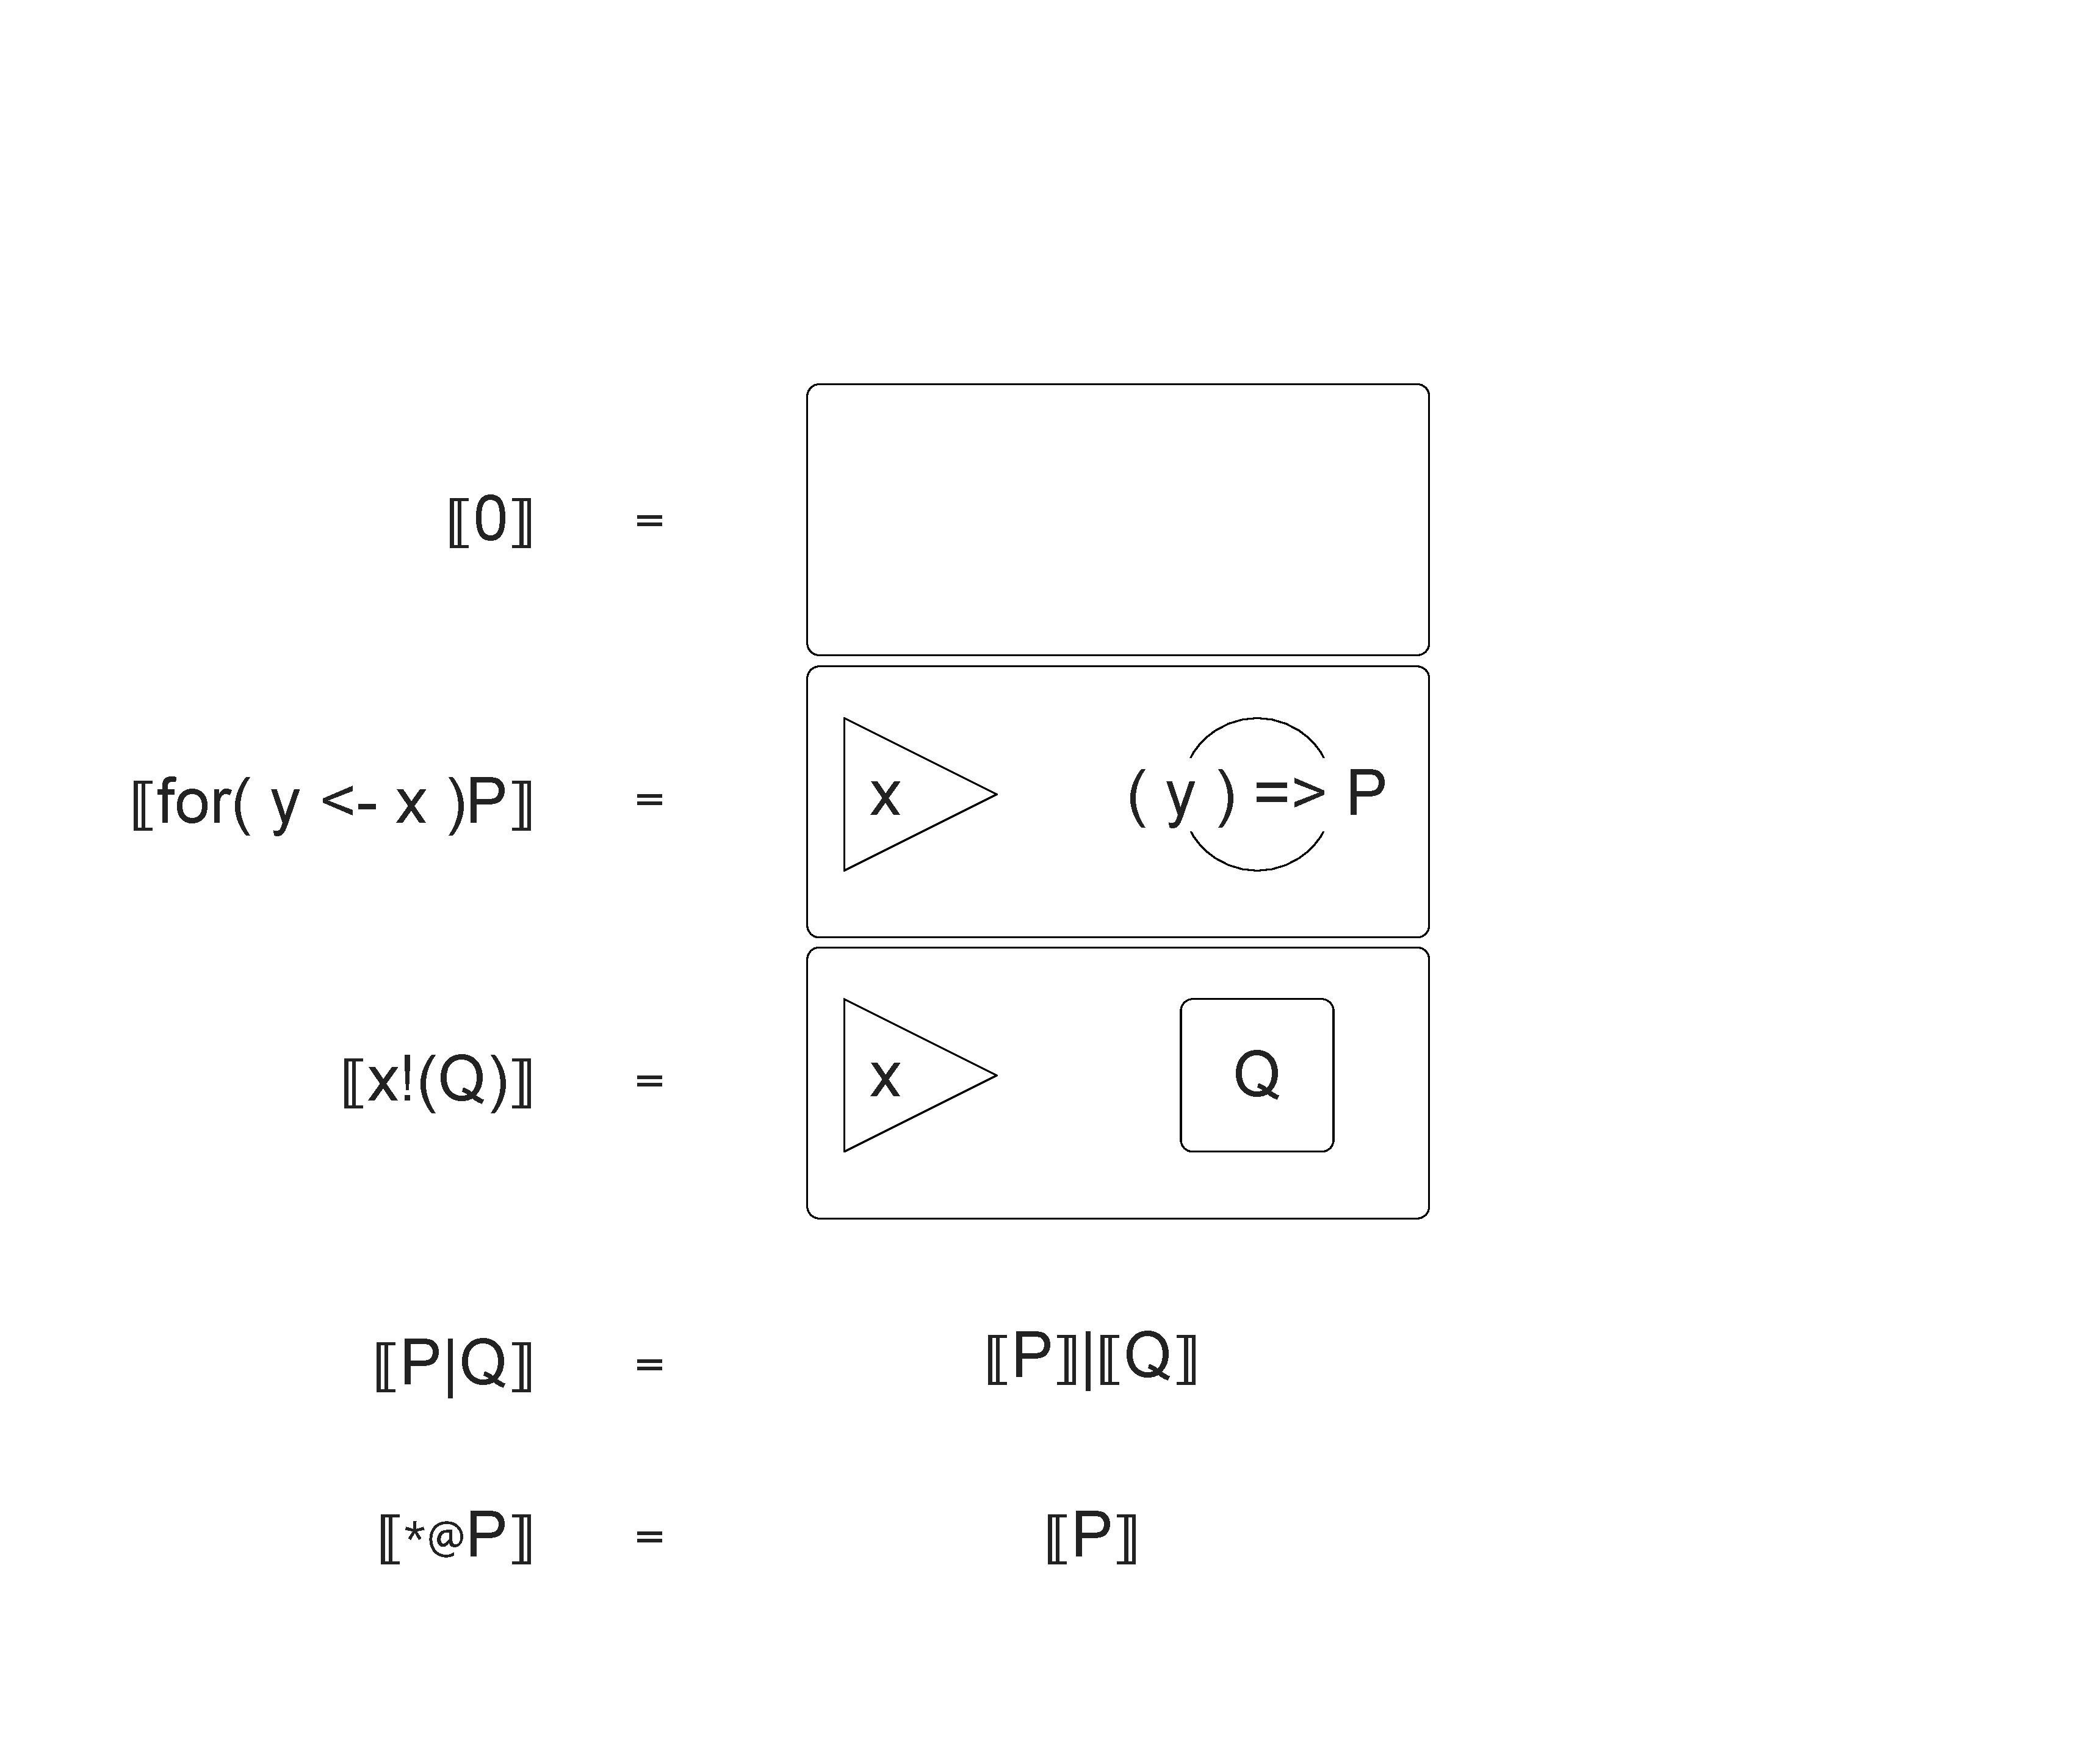
\includegraphics[scale=0.25]{RHO20RSpaceSlide1.pdf}

The diagram above indicates how to turn a given process state into an
$\mathsf{RSpace}$ instance. The 4th equation depends on an operation
on $\mathsf{RSpace}$ instances corresponding to parallel composition
of process states.

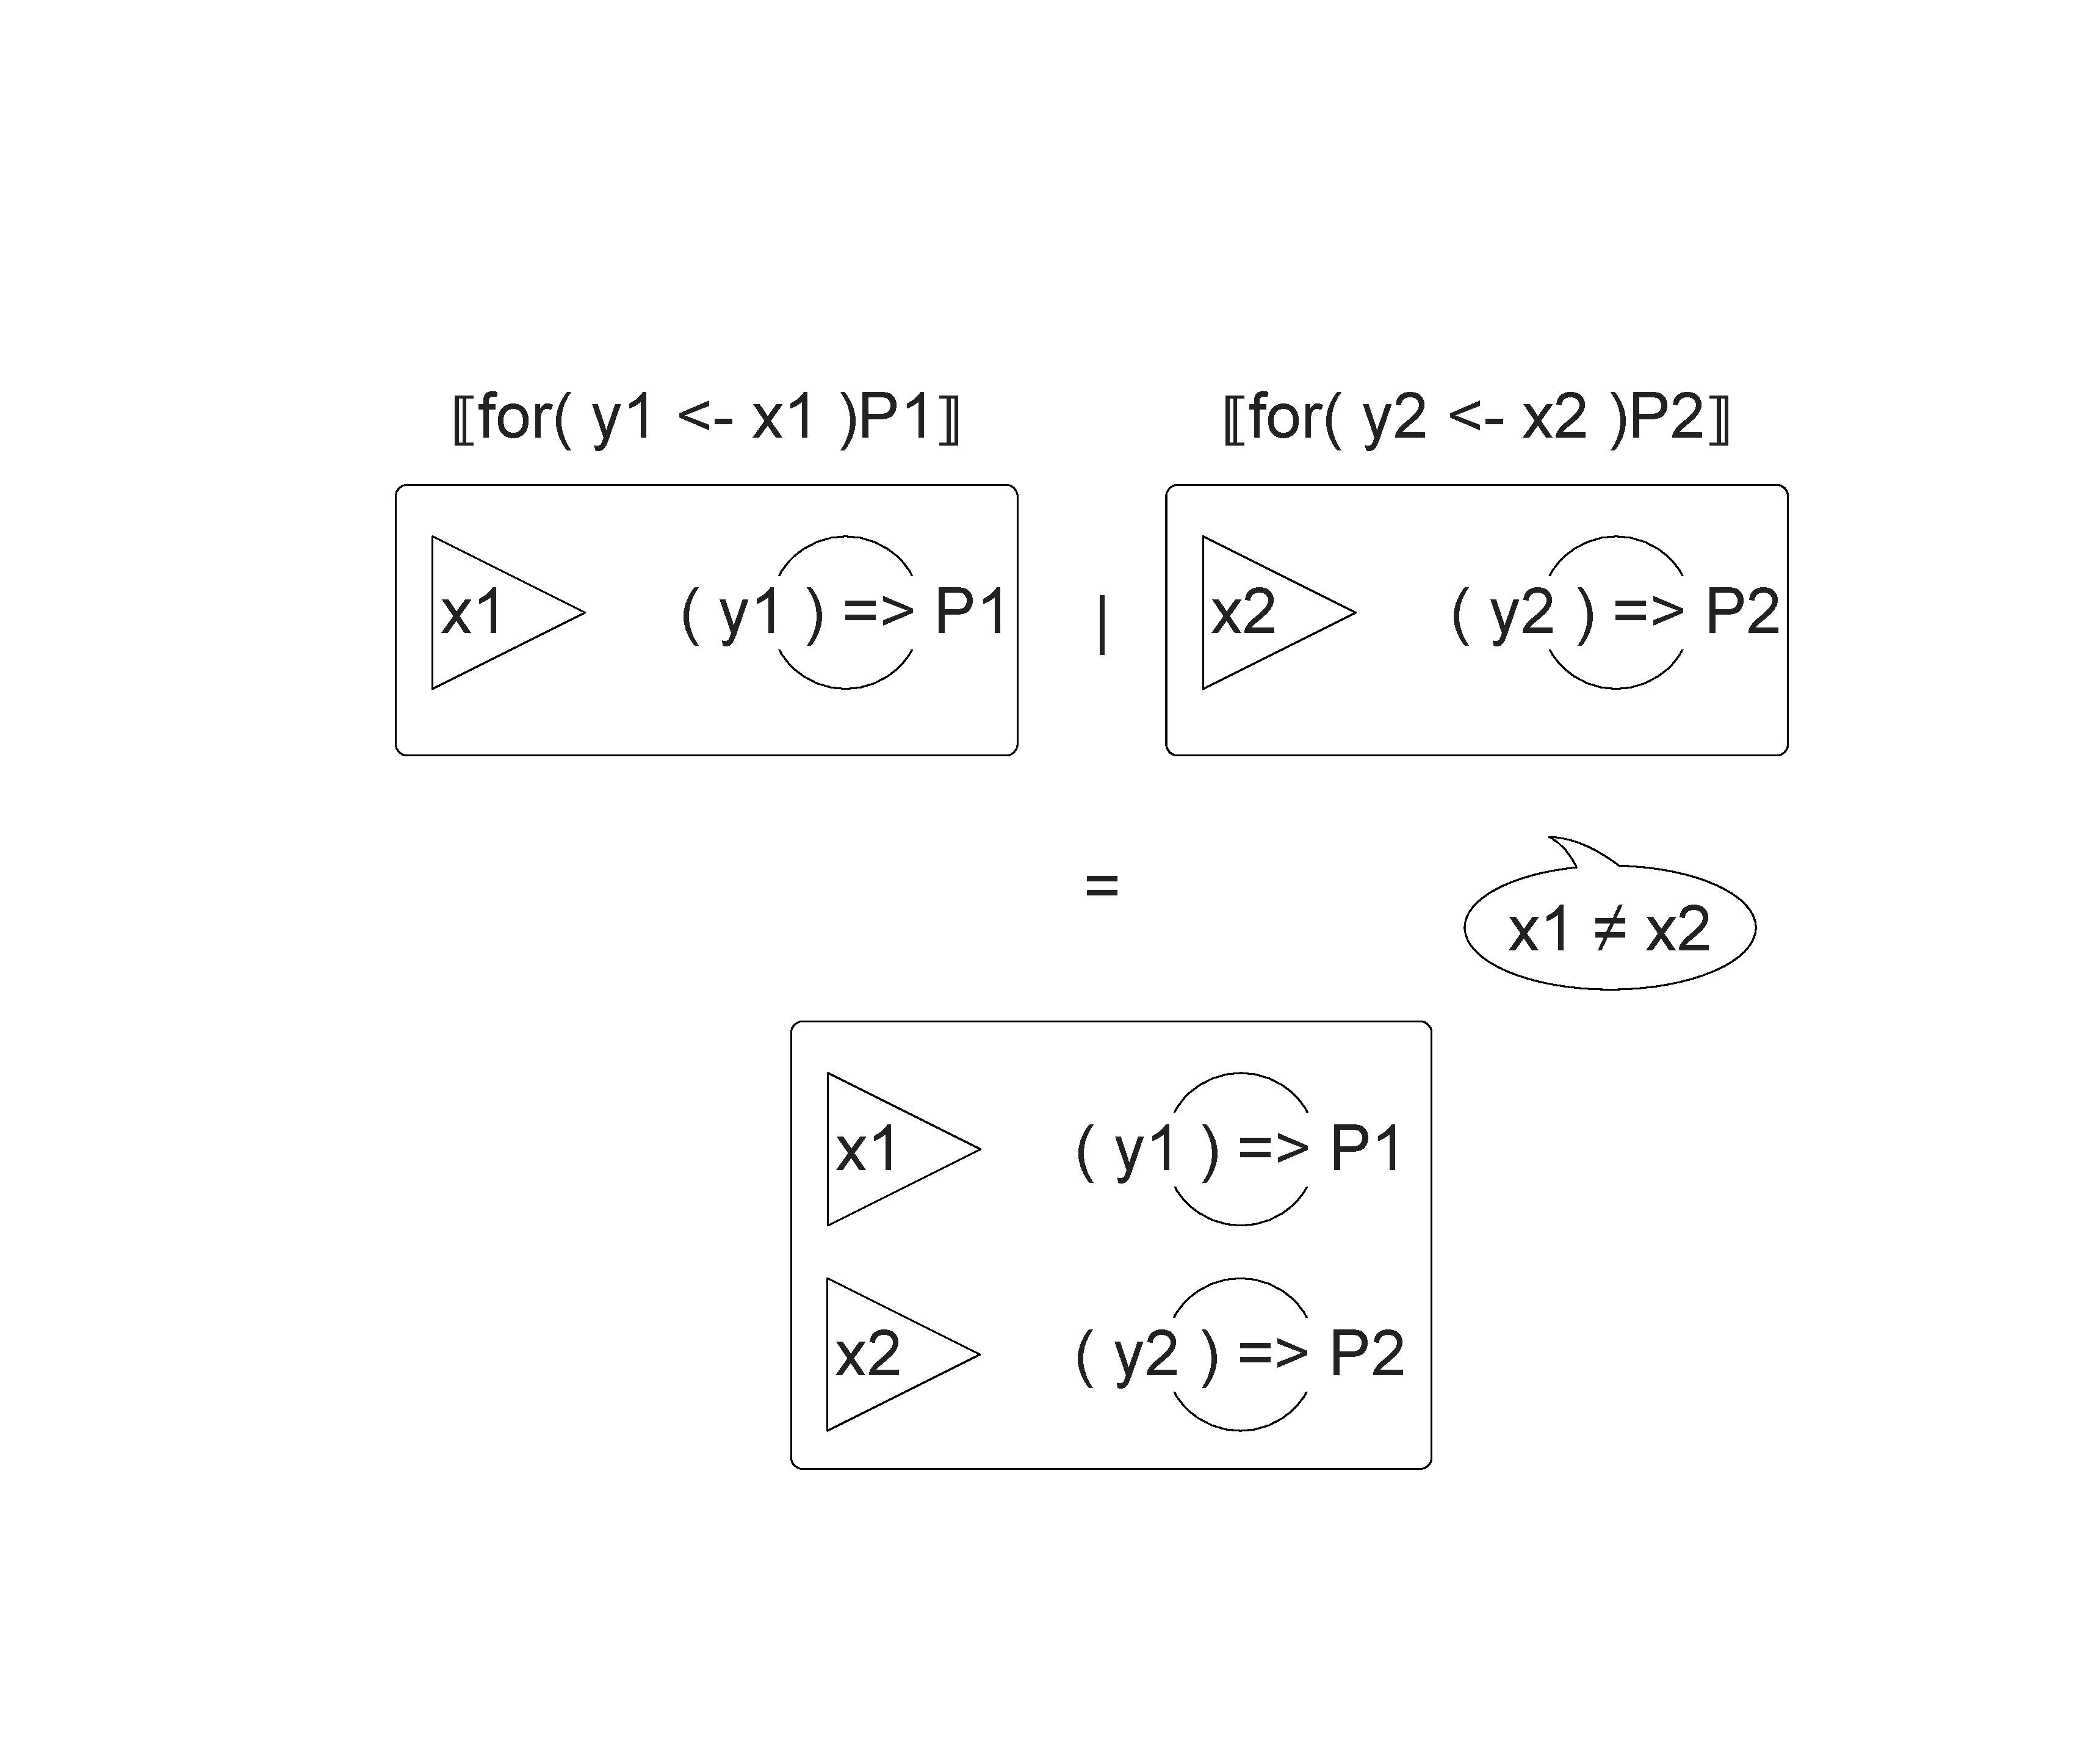
\includegraphics[scale=0.25]{RHO20RSpaceSlide2.pdf}

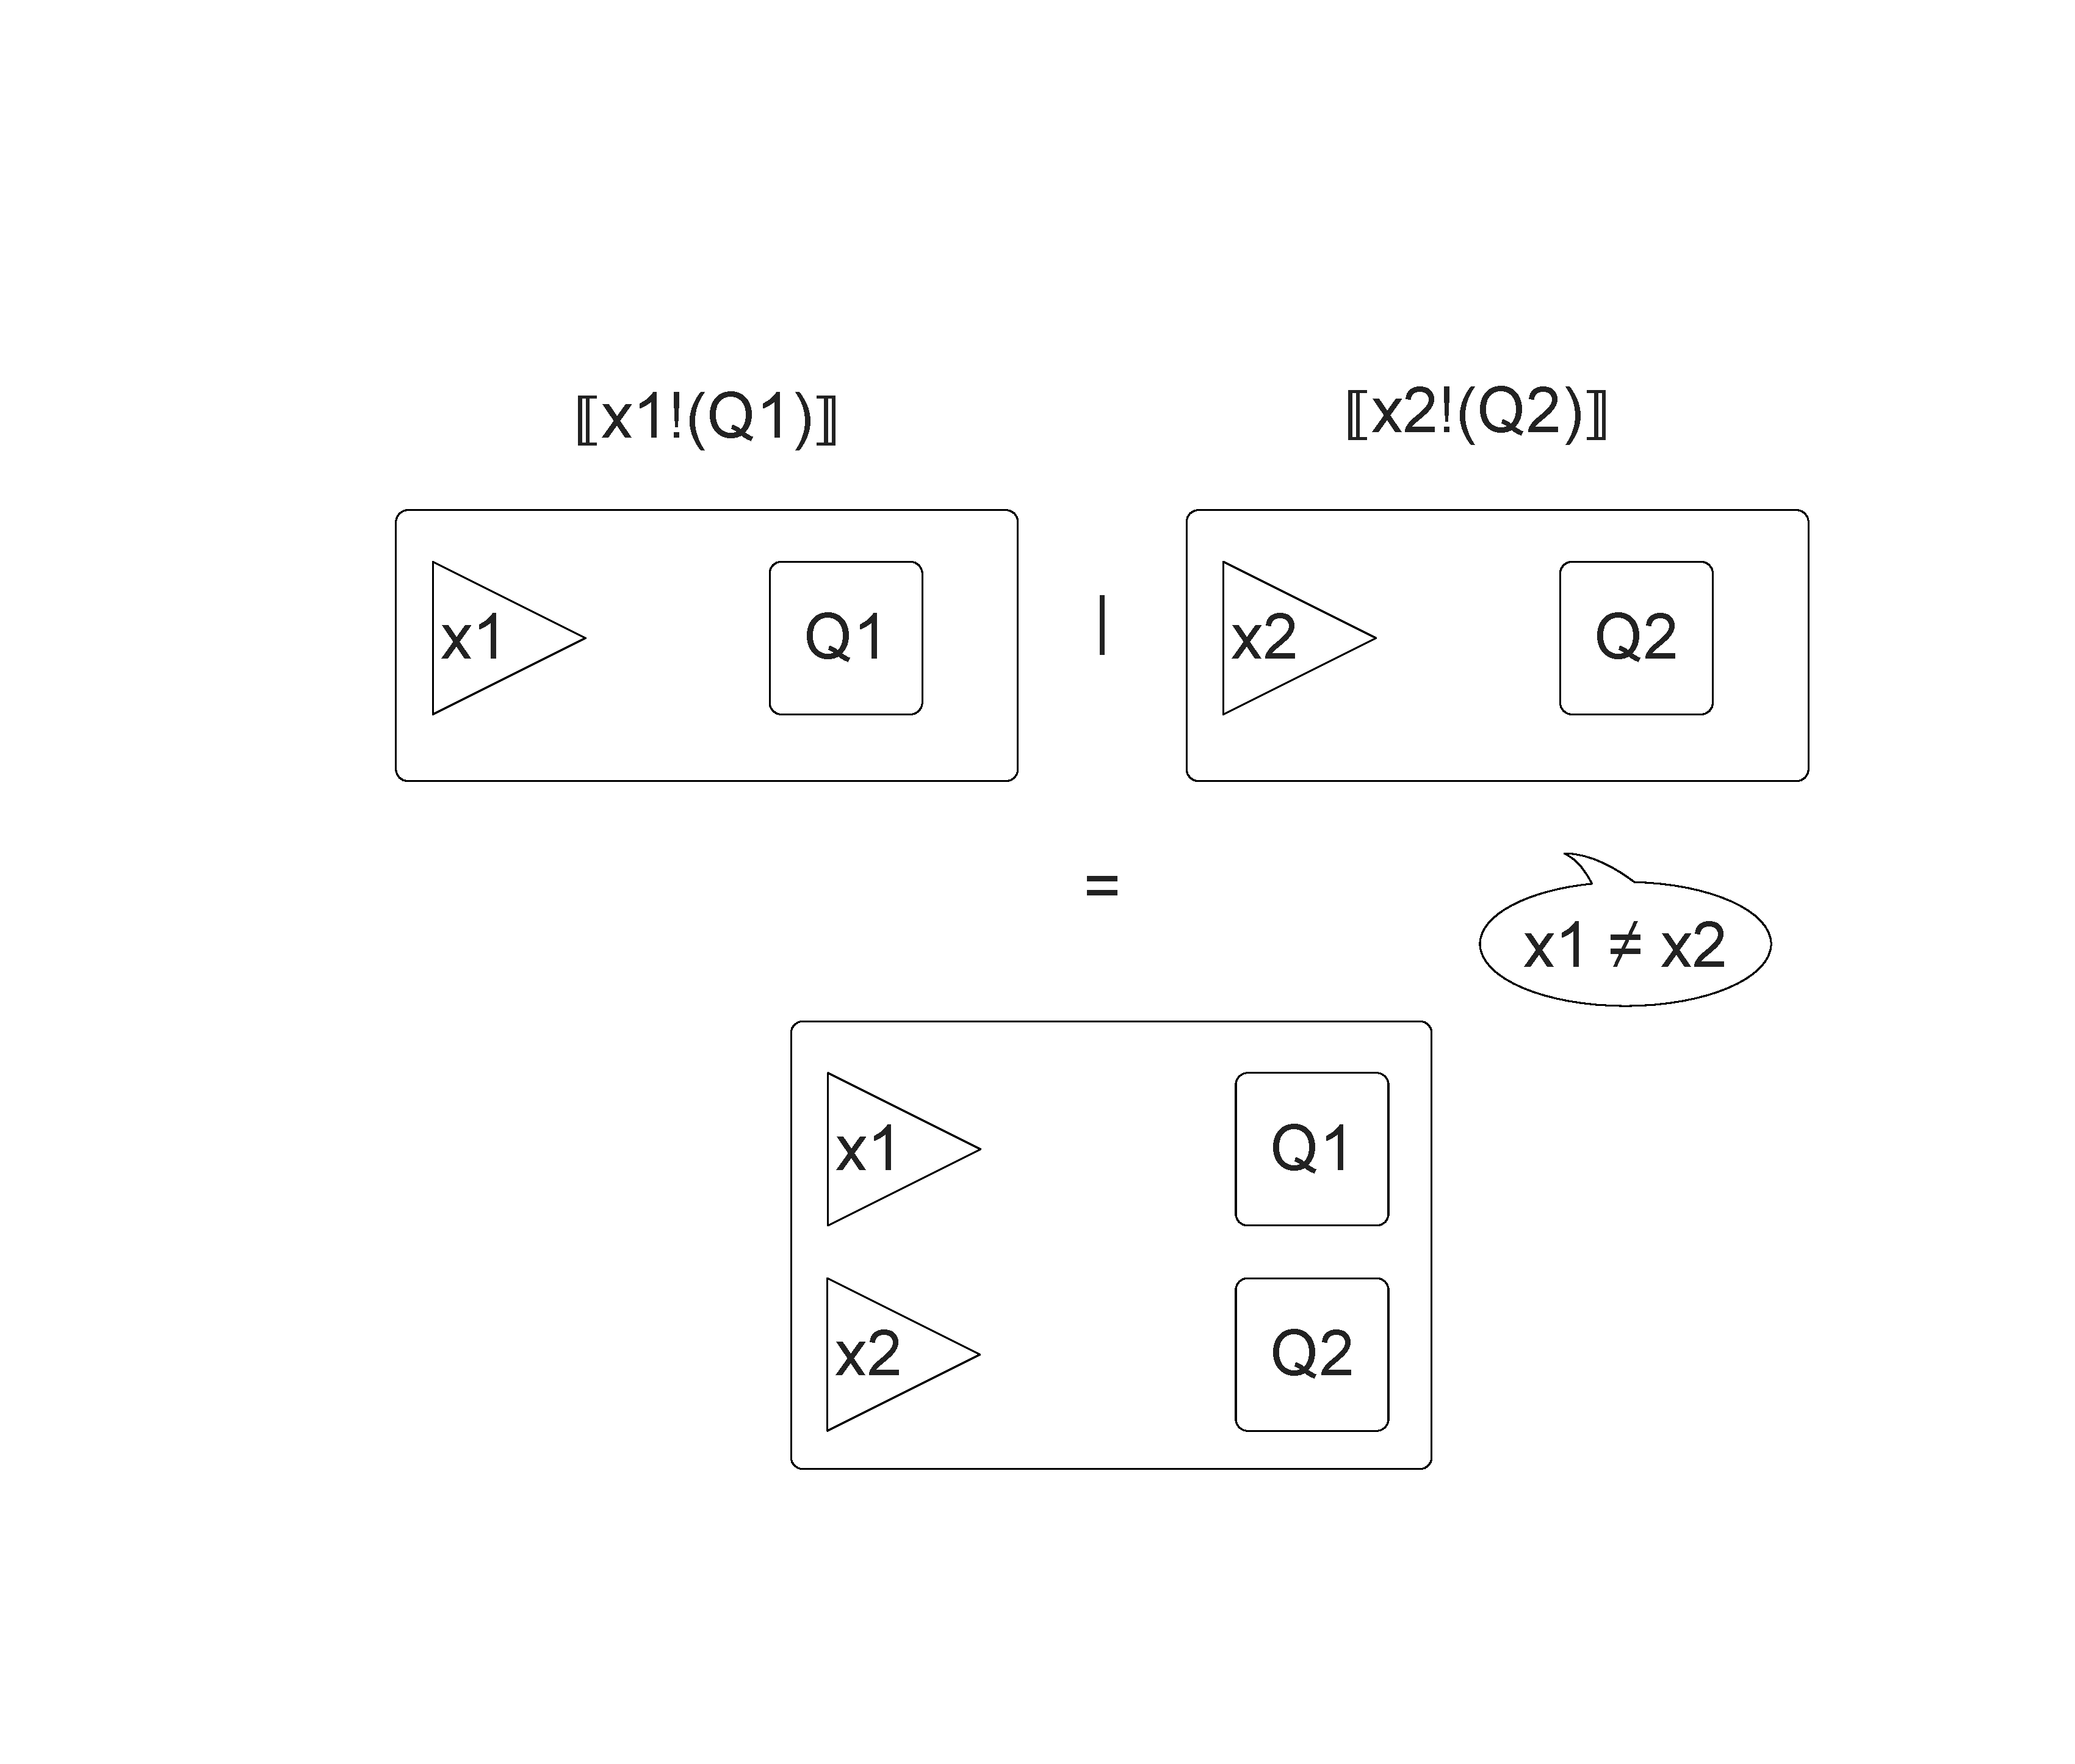
\includegraphics[scale=0.25]{RHO20RSpaceSlide3.pdf}

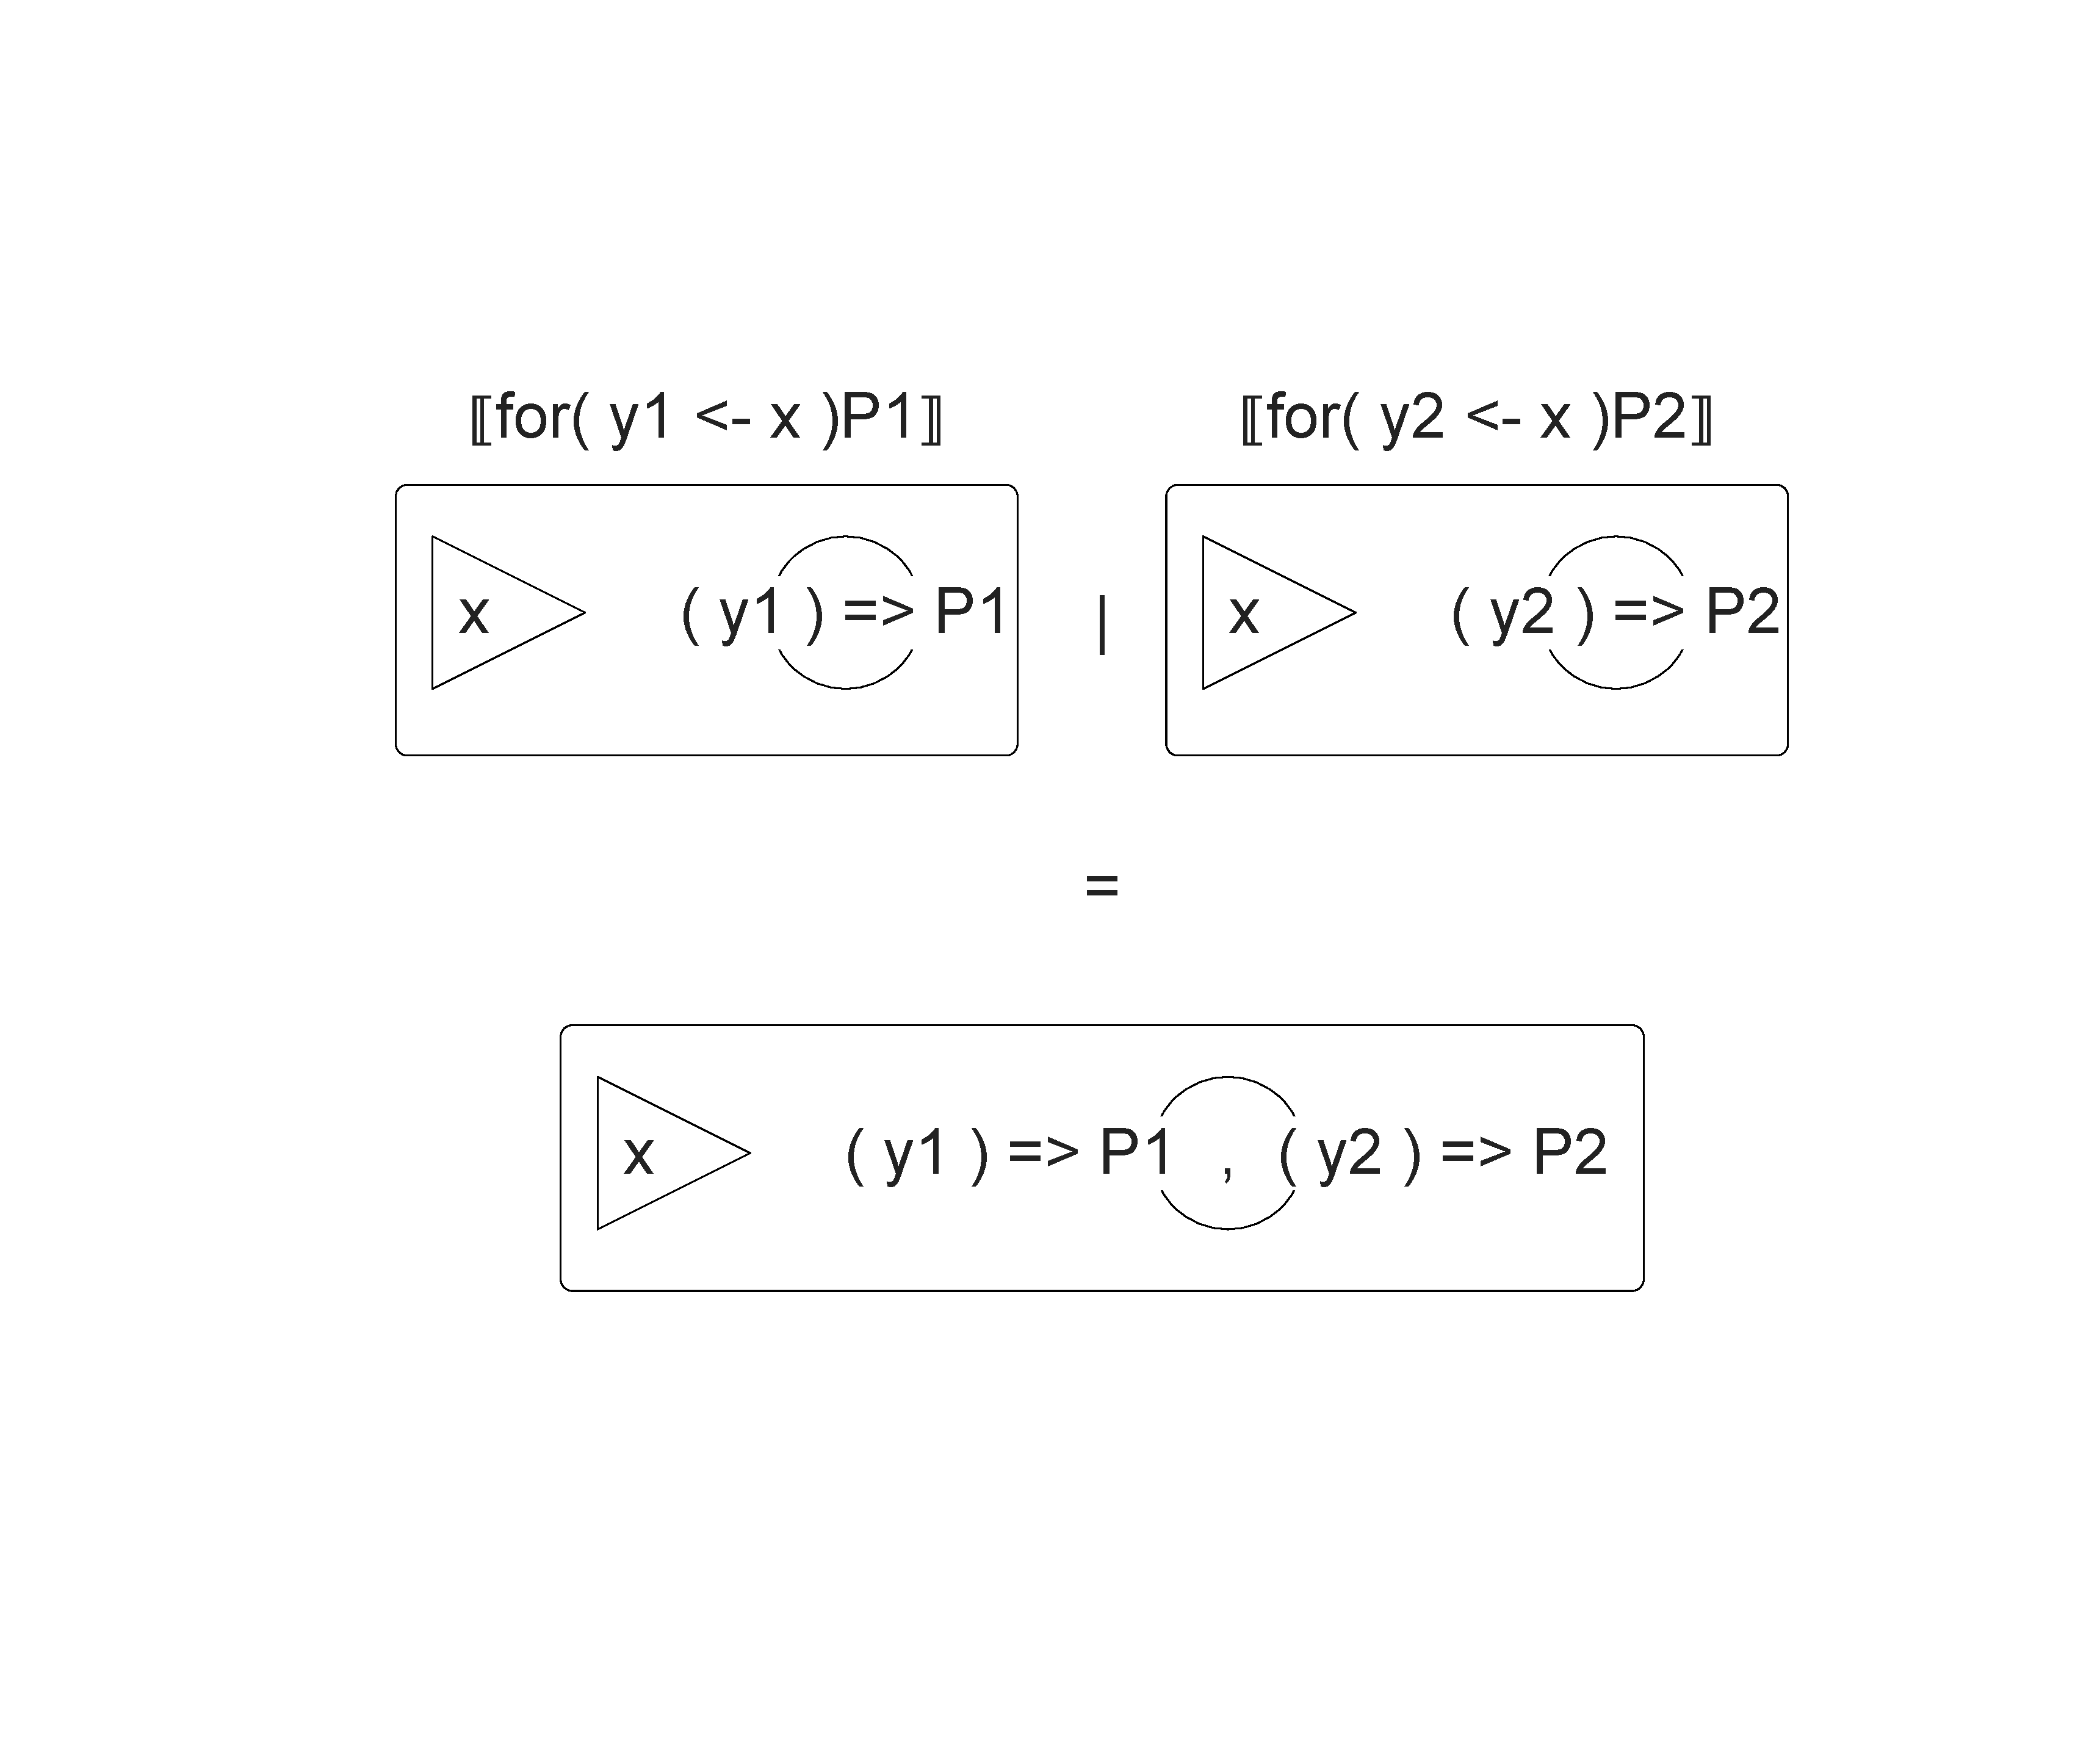
\includegraphics[scale=0.25]{RHO20RSpaceSlide4.pdf}

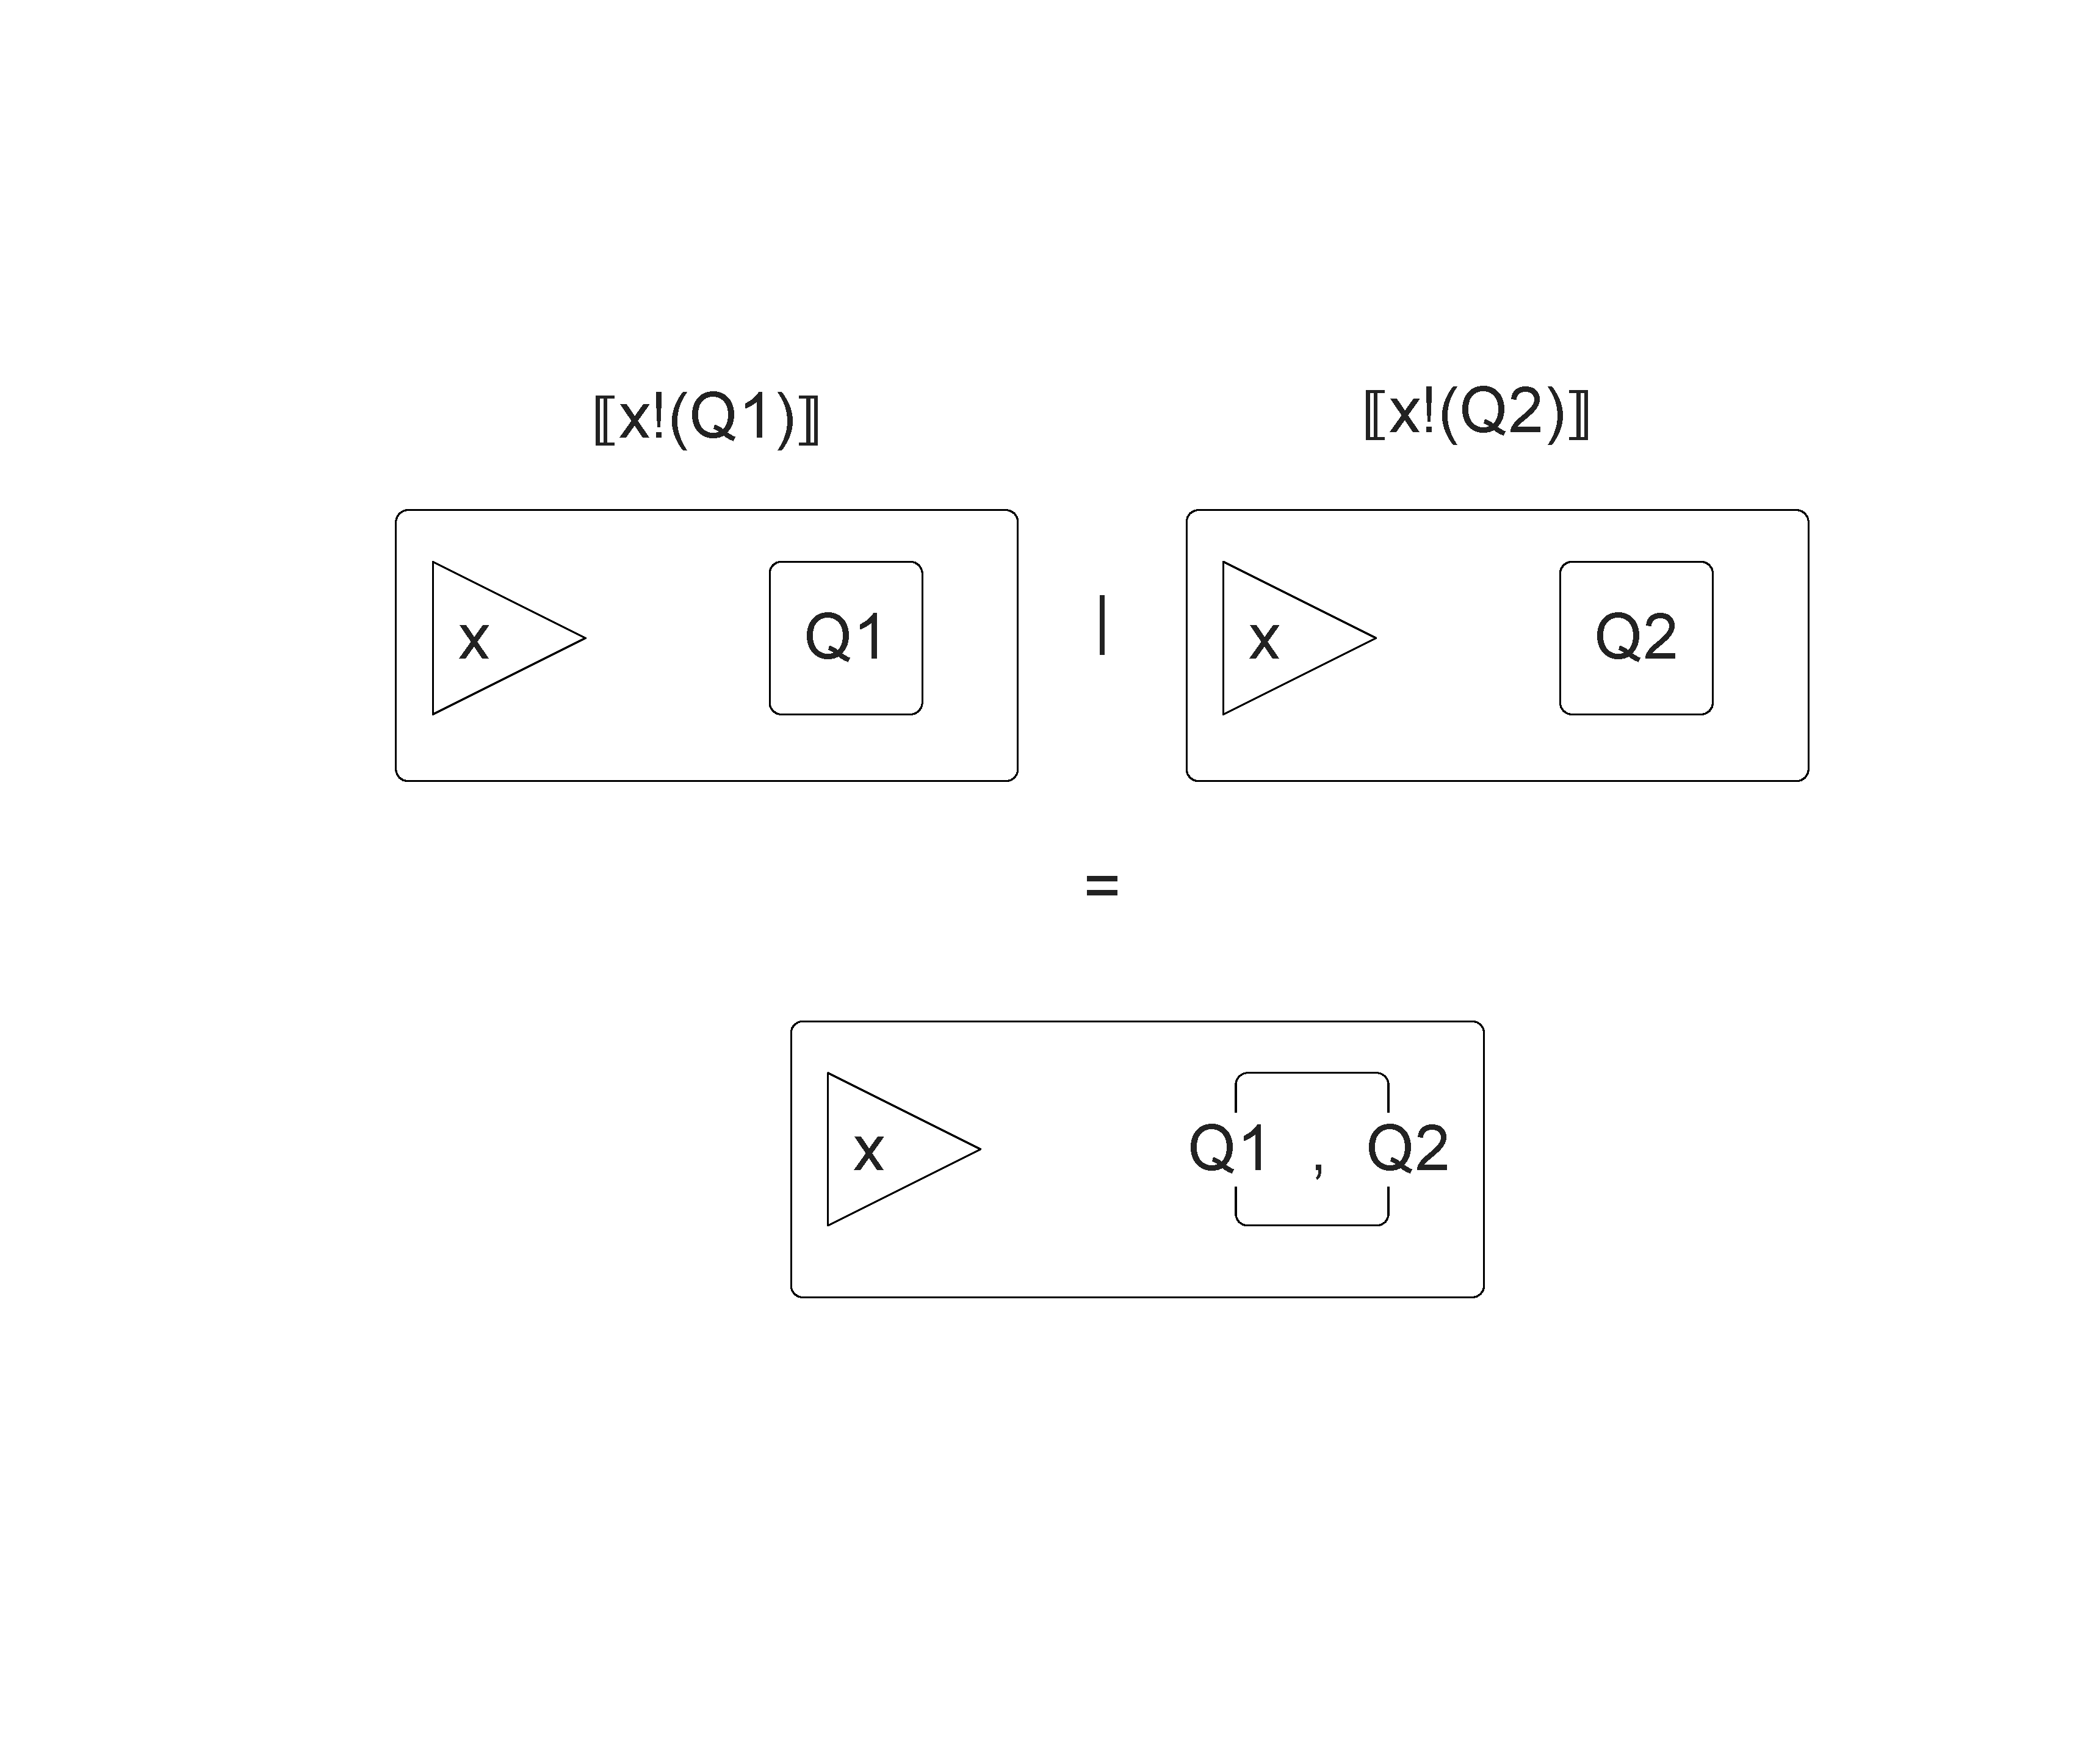
\includegraphics[scale=0.25]{RHO20RSpaceSlide5.pdf}

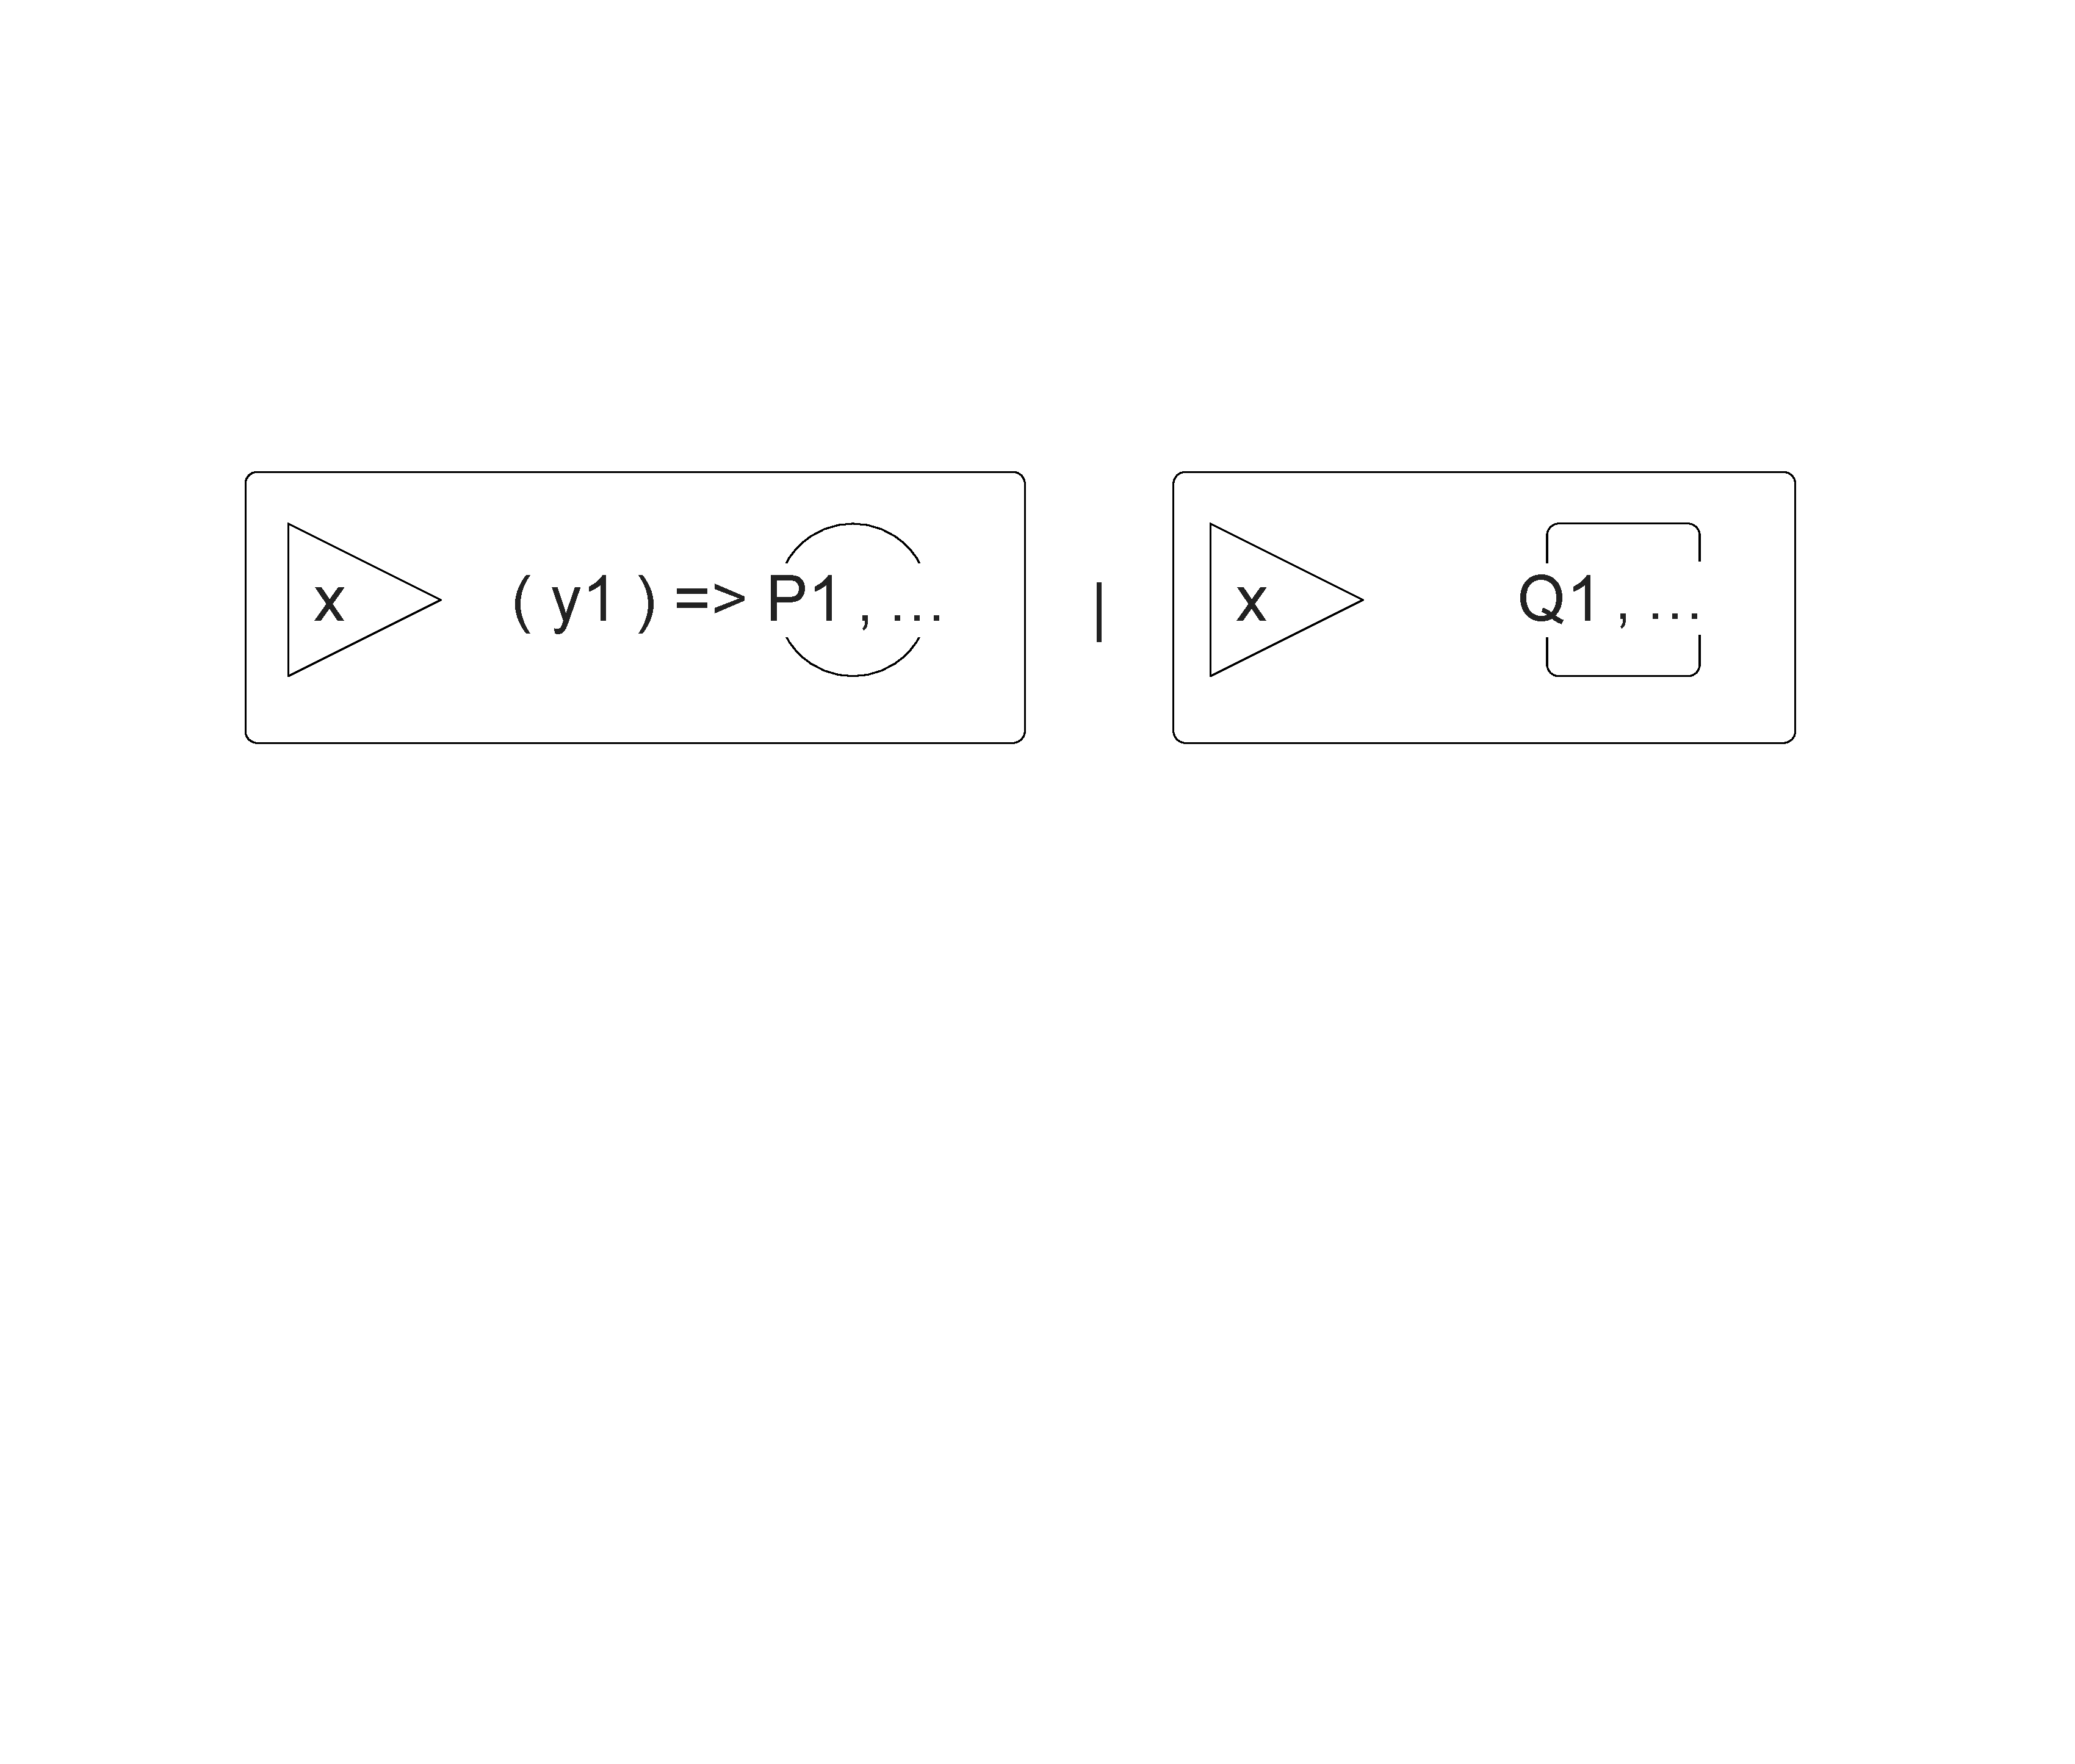
\includegraphics[scale=0.25]{RHO20RSpaceSlide6.pdf}

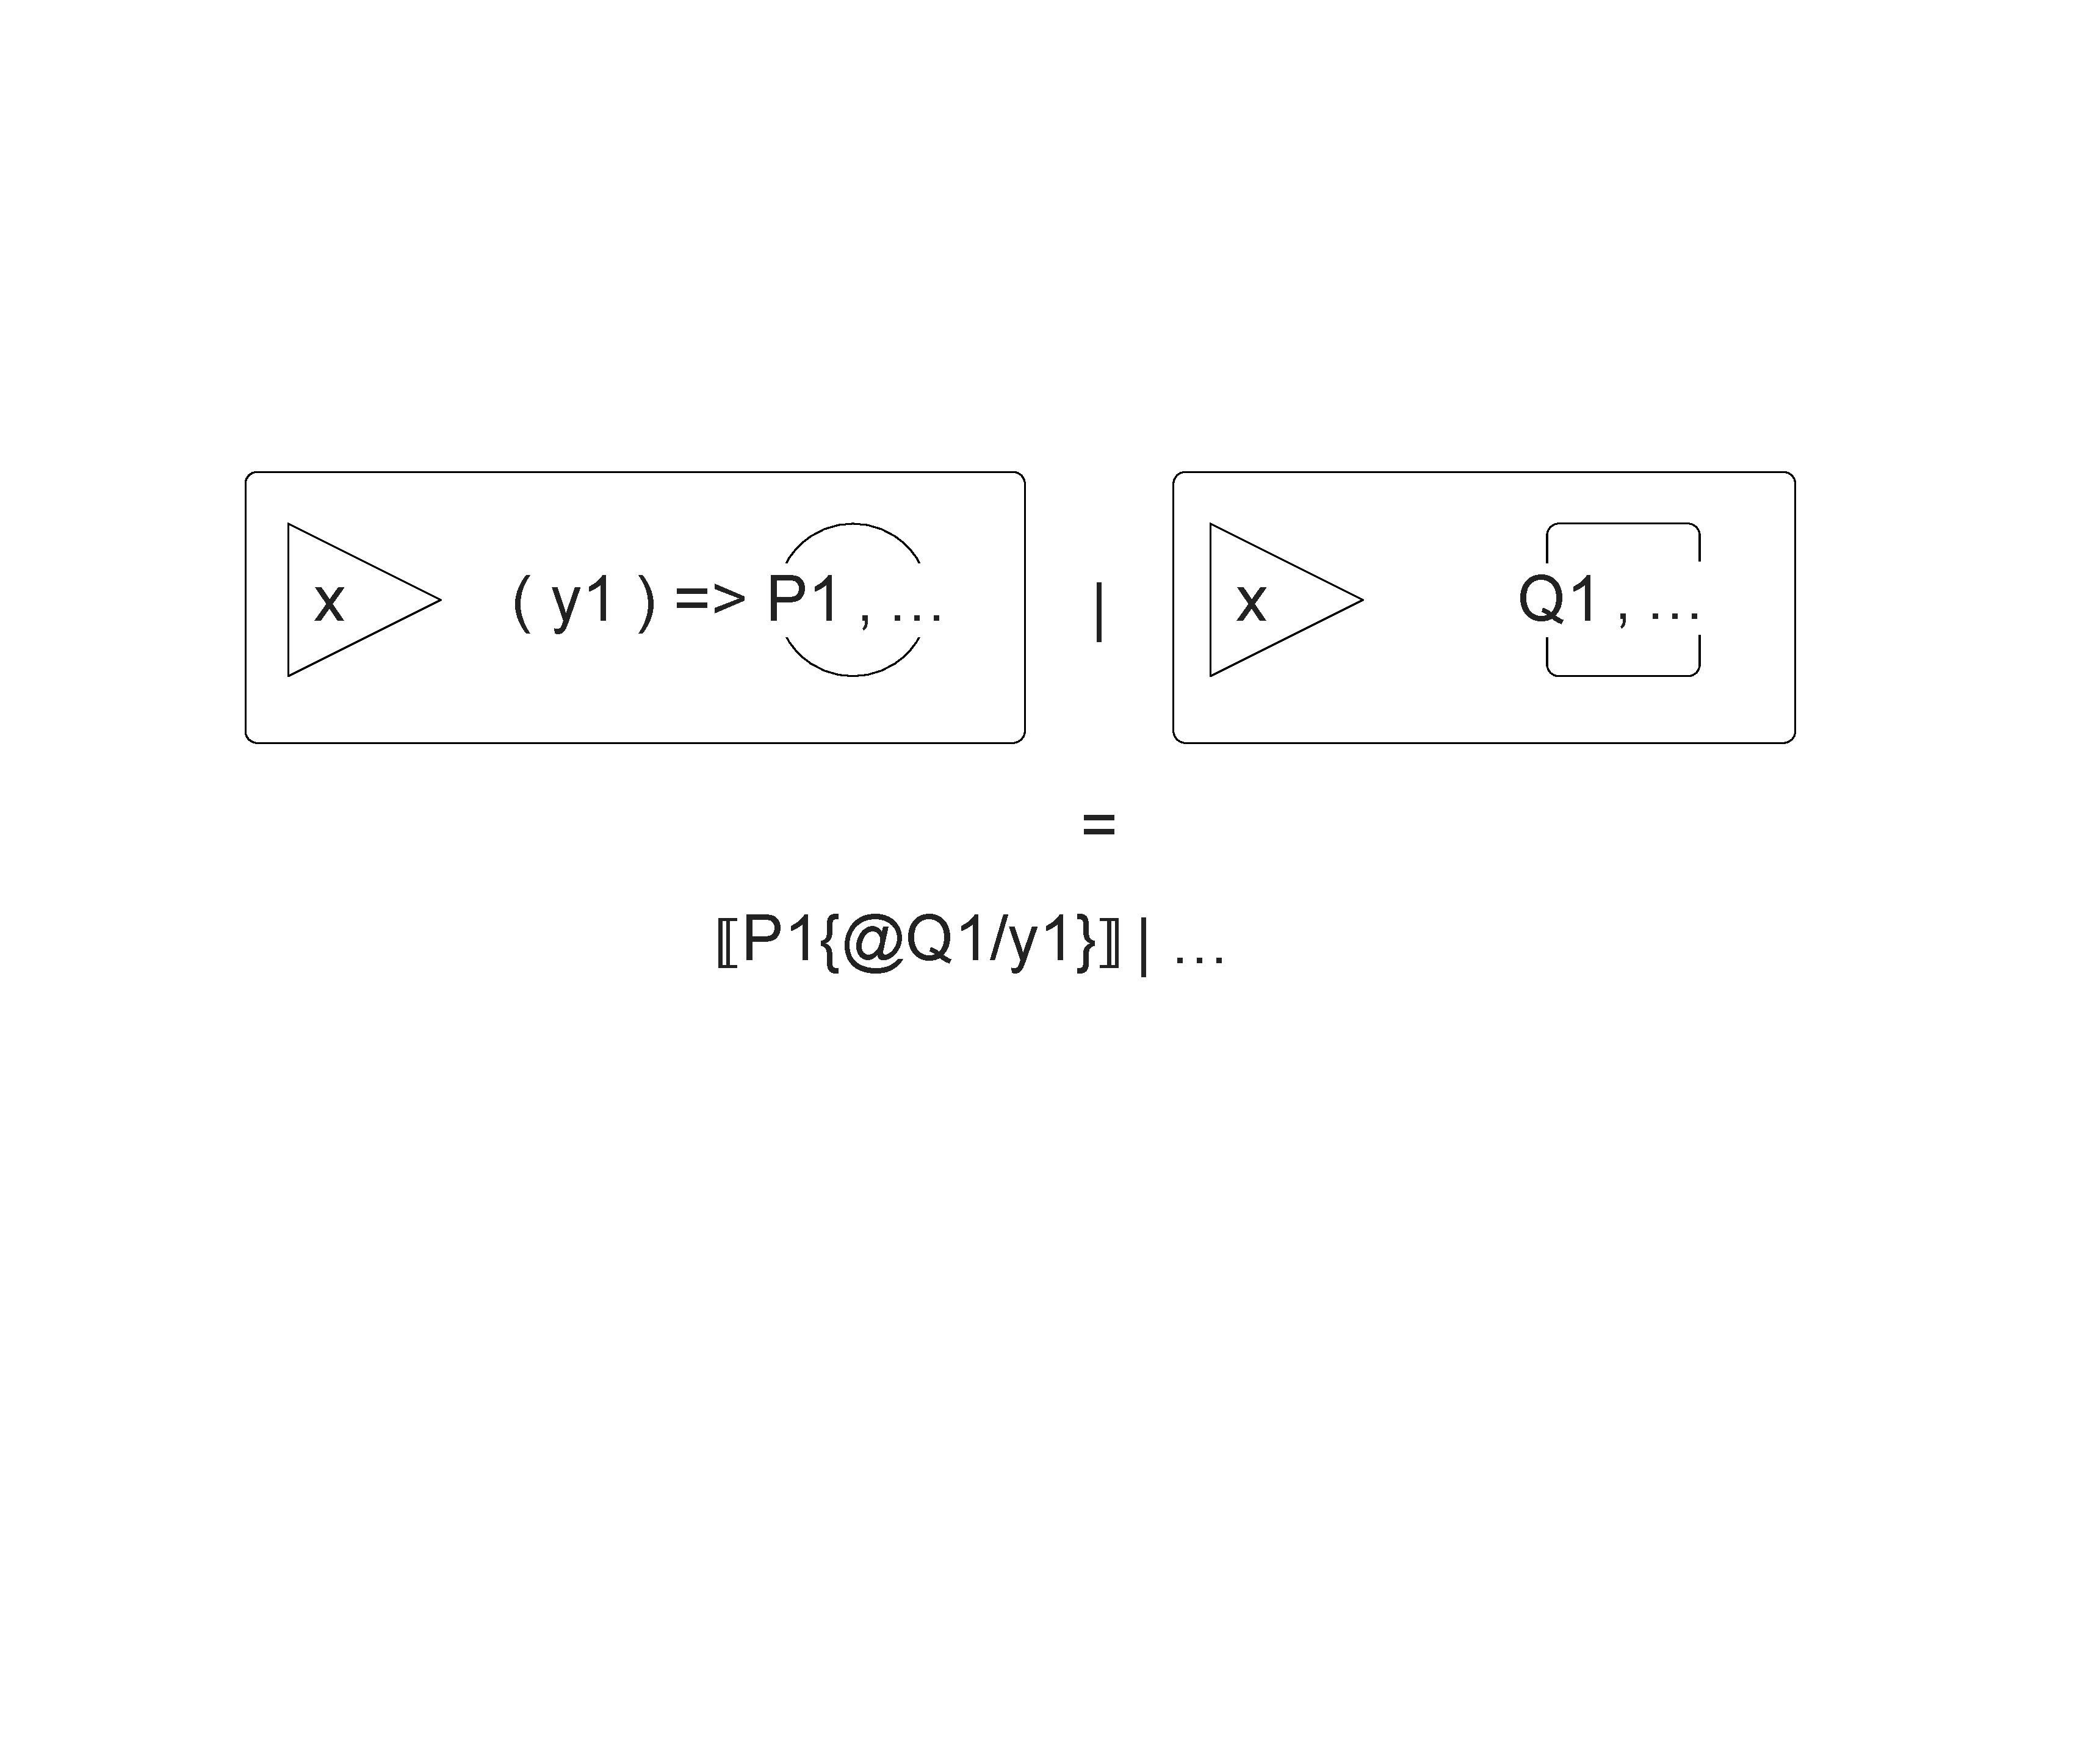
\includegraphics[scale=0.25]{RHO20RSpaceSlide7.pdf}

\subsection{Compiling rho to RSpace}

\begin{lstlisting}
  trait RhoRuntime {
     def execute( p : RPorQ )( r : RSpace ) : Unit = {
       p match {
         case Zero => { }
         case Input( x, y, p ) => { r.put( x, ( y ) => p ) }
         case Output( x, q ) => { r.put( x, Q ) }
         case Par( p, q ) => {
           val t1 = new Thread() {
             override def run() = { execute( p )( r ) } };
           val t2 = new Thread() {
             override def run() = { execute( q )( r ) }
           }; t1.run(); t2.run()
         }
         case Deref( Ref( p ) ) => { execute( p )( r ) } }
  } }
\end{lstlisting}

\subsubsection{Ordering rho terms}

TBD
